\section{Evaluation}

\subsection{Datengenerierung}
\label{datagen}

Der Vorgang der Datengenerierung wurde nach dem in Abbildung \ref{fig:overview2} aufgezeigten Schema implementiert. Durch die Verwendung einer Custom Map (zu Deutsch: \textit{benutzerdefinierten Karte}), eine durch den in StarCraft~II mitgelieferten Editor modifizierte Spielfläche, können die beiden Armeen mit zufällig zusammengestellten Einheiten-Konstellationen generiert werden. Zu Beginn des Gefechts werden beide Armeen am gegenseitigen Ende der Karte erzeugt. Bevor die Armeen den Kampf beginnen, wird der Spiel-Zustand (Spieler IDs, Höhenkarte, Einheitentyp, etc.) in Form von mehreren Matrix-Repräsentationen gespeichert. Sobald eine der beiden Seiten keine Einheiten mehr hat gilt die Schlacht als beendet und die Armee, welche noch über Einheiten verfügt wird als Sieger betrachtet. Das Ergebnis wird als Integer-Wert gespeichert und im späteren Verlauf des Trainings zu einem One-Hot-Vektor transformiert. 

Die Armeen werden zufällig generiert, der Generierungsprozess läuft wie folgt ab: Zunächst wird für beide Armeen eine Rasse gewürfelt. Die Rasse bestimmt welche Einheiten die Armee erzeugen darf. Im Folgenden wird für jede Einheit durch einen Zufallszahlen-Generator die Anzahl der maximal zu erzeugenden Einheiten ermittelt. Die Anzahl der Einheit, welche insgesamt von einer Armee erzeugt werden dürfen ist auf eine zufällige Grenze zwischen 10 und 50 begrenzt. Es werden daher alle Werte der einzelnen Einheiten so reduziert, dass die Gesamtzahl der Einheiten in einer Armee diese Grenze nicht überschreitet. Da bei zu großen Unterschieden in der Armeegröße die Klassifizierung zu einer trivialen Aufgabe wird, wurde zusätzlich eine Versorgungs-Grenze implementiert. In StarCraft~II ist die Versorgungsgrenzer ein Wert, welcher die Größe der Armee eines Spieler begrenzt. Diese Grenze wird in dem Kontext der Datengenerierung genutzt um nur jene Gefechte zu erzeugen, in denen der Unterschied der Einheiten-Versorgung (folgend Supply-Differenz) beider Armeen kleiner ist als ein definierter Grenzwert (in diesem Fall 5).

Abbildung \ref{fig:overview1} zeigt den Generierungsprozess in Gänze. Die Custom Map aus StarCraft~II generiert ein Gefecht mit passender Differenz an Einheiten-Versorgung und lässt dieses nach speichern des Spielzustands austragen. Dieser Vorgang wird vor dem Beenden der Custom Map 25 Mal ausgeführt. Mit Beenden der Custom Map werden alle Vorgänge auf der Karte, als Replay (zu Deutsch: \textit{Wiederholung}) gespeichert. Ein Replay enthält somit 25 Gefechte, welche alle einzeln ausgewertet werden. 

Die Entscheidung mehrere Gefechte auf einmal zu generieren wurde getroffen, da die Custom Map bei jedem Start das Spiel neu laden muss und somit der zeitliche Overhead bei Einzelgenerierung der Replays wesentlich größer wäre. Die Anzahl der in einem Replay generierten Gefechte wurde auf 25 gesetzt, da bei zu vielen Iterationen der Gefechtsgenerierung die Replay-Datei zu groß wurde und das Spiel beim Schließen der Custom Map abstürzte. Der Absturz resultierte in jedem Fall in einem Datenverlust. Bei 25 Gefechten pro Replay liegt die Absturzrate derzeit immer noch bei ca. 50\%, jedoch resultierte das weitere Senken der Gefechte pro Replay nicht in einem stabileren Generationsprozess. 

Die Generierung der Gefechte findet auf der schnellsten Spieleinstellung statt, damit in gleicher Zeit mehr Gefechte simuliert werden können. Dadurch ist es aktuell möglich in einem Zeitraum von acht Stunden ca. 250 valide (500 Generierungen inklusive der Abstürze) Replays zu produzieren, welche nach der Feature Extraktion (Zeitaufwand erneut ca. drei bis vier Stunden) in 6250 Samples resultieren. 

\newpage
\begin{figure}[H]
\thispagestyle{empty}
\centering
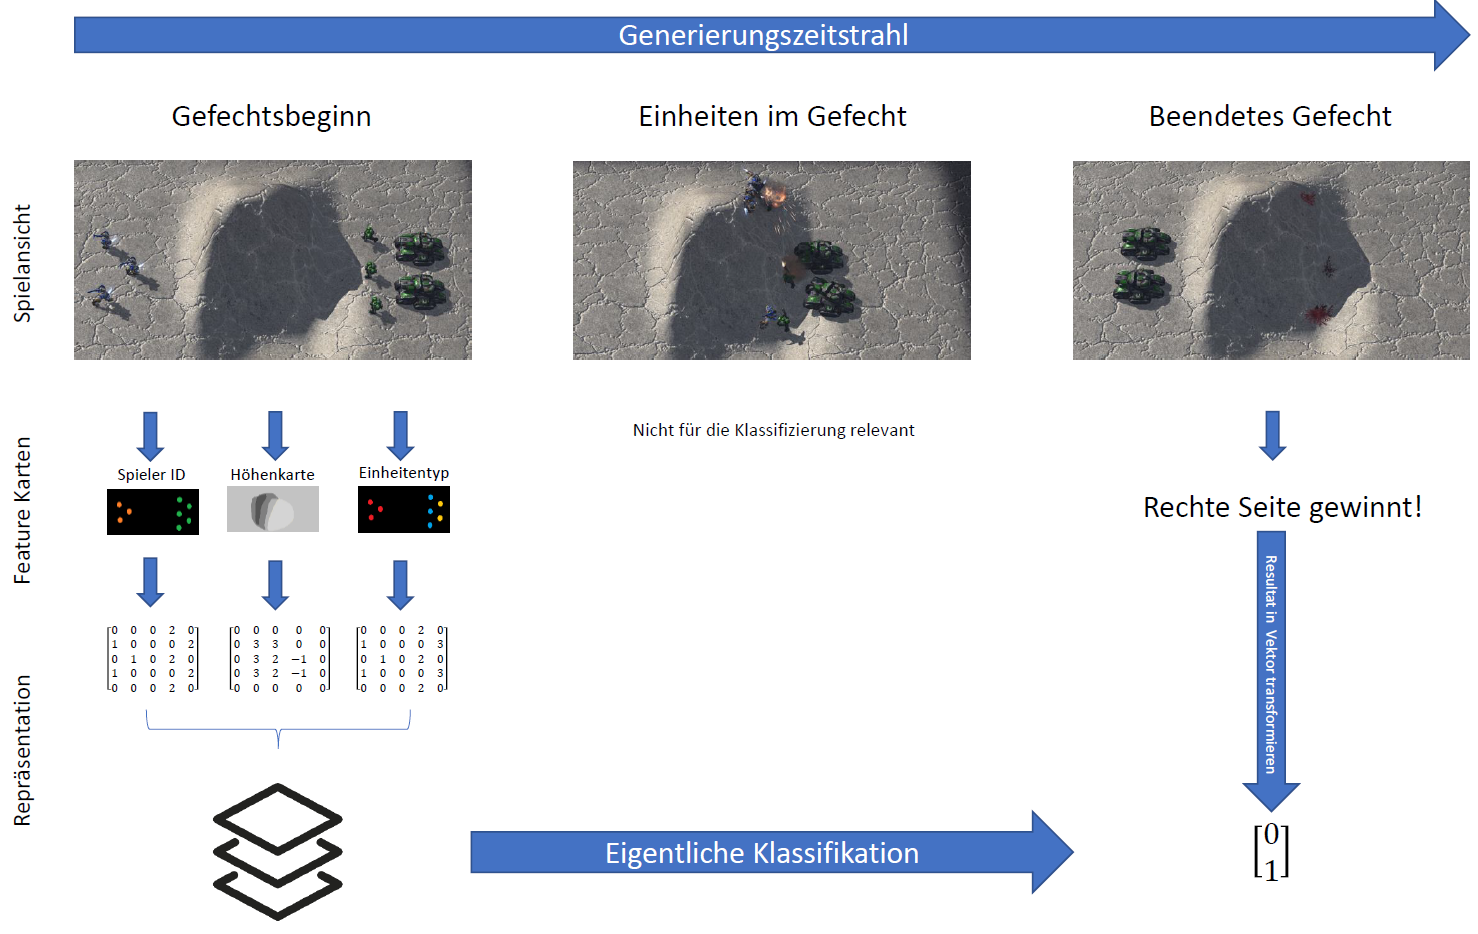
\includegraphics[angle=90,scale=0.6]{pictures/grafiken/Folie1}
\caption{Übersicht des Generierungsprozesses der Trainingsdaten.}
\label{fig:overview2}
\end{figure}

\begin{figure}[H]
\thispagestyle{empty}
\centering
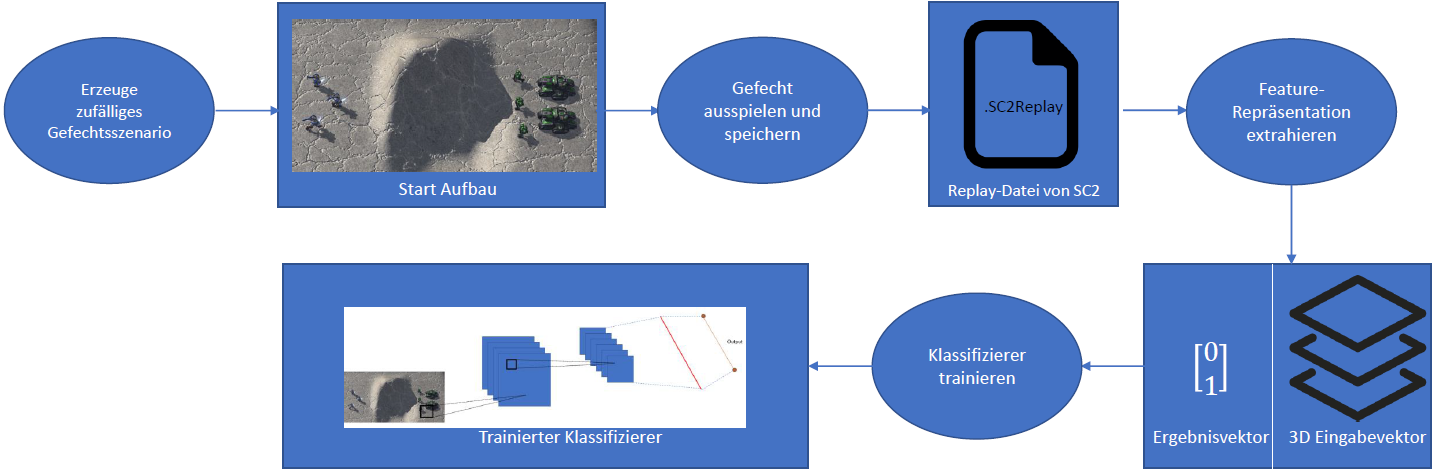
\includegraphics[angle=90,scale=0.6]{pictures/grafiken/Folie2}
\caption{Übersicht des Generierungsprozesses der Trainingsdaten.}
\label{fig:overview1}
\end{figure}

Die Abbildungen \ref{fig:suppvert}, \ref{fig:siegvert} und \ref{fig:siegsupp} zeigen die Zusammensetzung der simulierten Gefechte auf. Abbildung \ref{fig:suppvert} zeigt die absolute Anzahl der Gefechte unter Berücksichtigung der Supply-Differenz. Die X-Achse trägt die Supply-Differenz in 0,5er-Schritten auf und auf der Y-Achse befindet sich die absolute Anzahl der entsprechenden Gefechte. Um die reelle Differenz der Gefechte zu erhalten muss man den Wert der X-Achse durch zwei teilen. Es sind drei klare Abstufungen zu erkennen. Die meisten Gefechte wurden mit einer Supply-Differenz $sd \leq 5$ generiert. Das zweite Plateau bilden die Gefechte $5 < sd \leq 10$ und das dritte Plateau wird von den Gefechten mit $10 < sd \leq 15$  gebildet. Die Bildung der Plateau ist durch den Generierungsprozess zu erklären. Es wurden mittels drei unterschiedlicher Custom Maps Daten generiert, welche in Versionen unterteilt wurden. Die erste Version lässt die Generierung von Gefecht mit einer Differenz von bis zu 5 zu. Version 2 lässt eine Differenz von 10 zu und Version 3 dementsprechend von 15. Da engere Gefechte nicht ausgeschlossen wurden, ist die Anzahl der engen Differenzen folglich höher. Die starken Einbrücke in jedem zweiten Balken werden von der Rasse \textit{Zerg} hervorgerufen, da diese die einzige Rasse sind deren Einheiten eine Supply-Anforderung von 0,5 haben können. Somit sind auch Differenzen mit X,5 nur möglich bei einer Beteiligung der Zerg an dem Gefecht. Auch wenn die Versionen nur Gefechte mit einer Differenz von maximal 15 zulassen, wurden dennoch Gefechte mit teilweise deutlich höheren Differenzen generiert. Dieser Umstand ist der Tatsache geschuldet, dass die Custom Maps während der Generierung bei einer zu großen Supply-Differenz die Armeen neu würfeln. Wenn dieser Vorgang zu oft wiederholt werden muss, kommt es zu einem Absturz der Custom Map, weshalb nach 8  Wiederholungen das Gefecht ohne Berücksichtigung der Supply-Differenz generiert wird um einem Absturz zu verhindern. Da die Supplies auch gespeichert werden, können diese Gefechte beim Training der Modelle problemlos herausgefiltert werden. 

\begin{figure}[H]
\centering
\includegraphics[scale=0.4]{pictures/Match_verteilung}
\caption{Verteilung der generierten Gefechte nach Supply-Differenz.}
\label{fig:suppvert}
\end{figure}

Abbildung \ref{fig:siegvert} zeigt die Anzahl der Gefechte, sowie die Anzahl der Siege insgesamt und nach gegnerischer Rasse. Die drei Balkengruppen sind nach Rassen aufgeteilt und zeigen für jede Rasse jeweils die Anzahl der Gefechte, Siege, Siegen gegen Zerg, Protoss und Terran. Die Anzahl der Gefechte ist für alle Rassen in etwa gleich und liegt zwischen 81.000 (Zerg) und 85.500 (Terran). Die Siege sind auch in ähnlichen Dimensionen, wobei Protoss und Terran mit jeweils 38.000 Siegen sehr nah beieinander liegen und Zerg mit 44.000 etwas darüber. Die Siege nach Rassen weisen im allgemeinen eine gleichmäßige Verteilung auf. Lediglich beim Aufeinandertreffen von Protoss und Terran scheinen die Protoss einen Vorteil zu haben, da die Terraner nur einen Bruchteil der Siege gegen Protoss haben. Protoss gewann 15.719 mal gegen Terran, Terran hingegen nur 4263 mal gegen Protoss.

\begin{figure}[H]
\centering
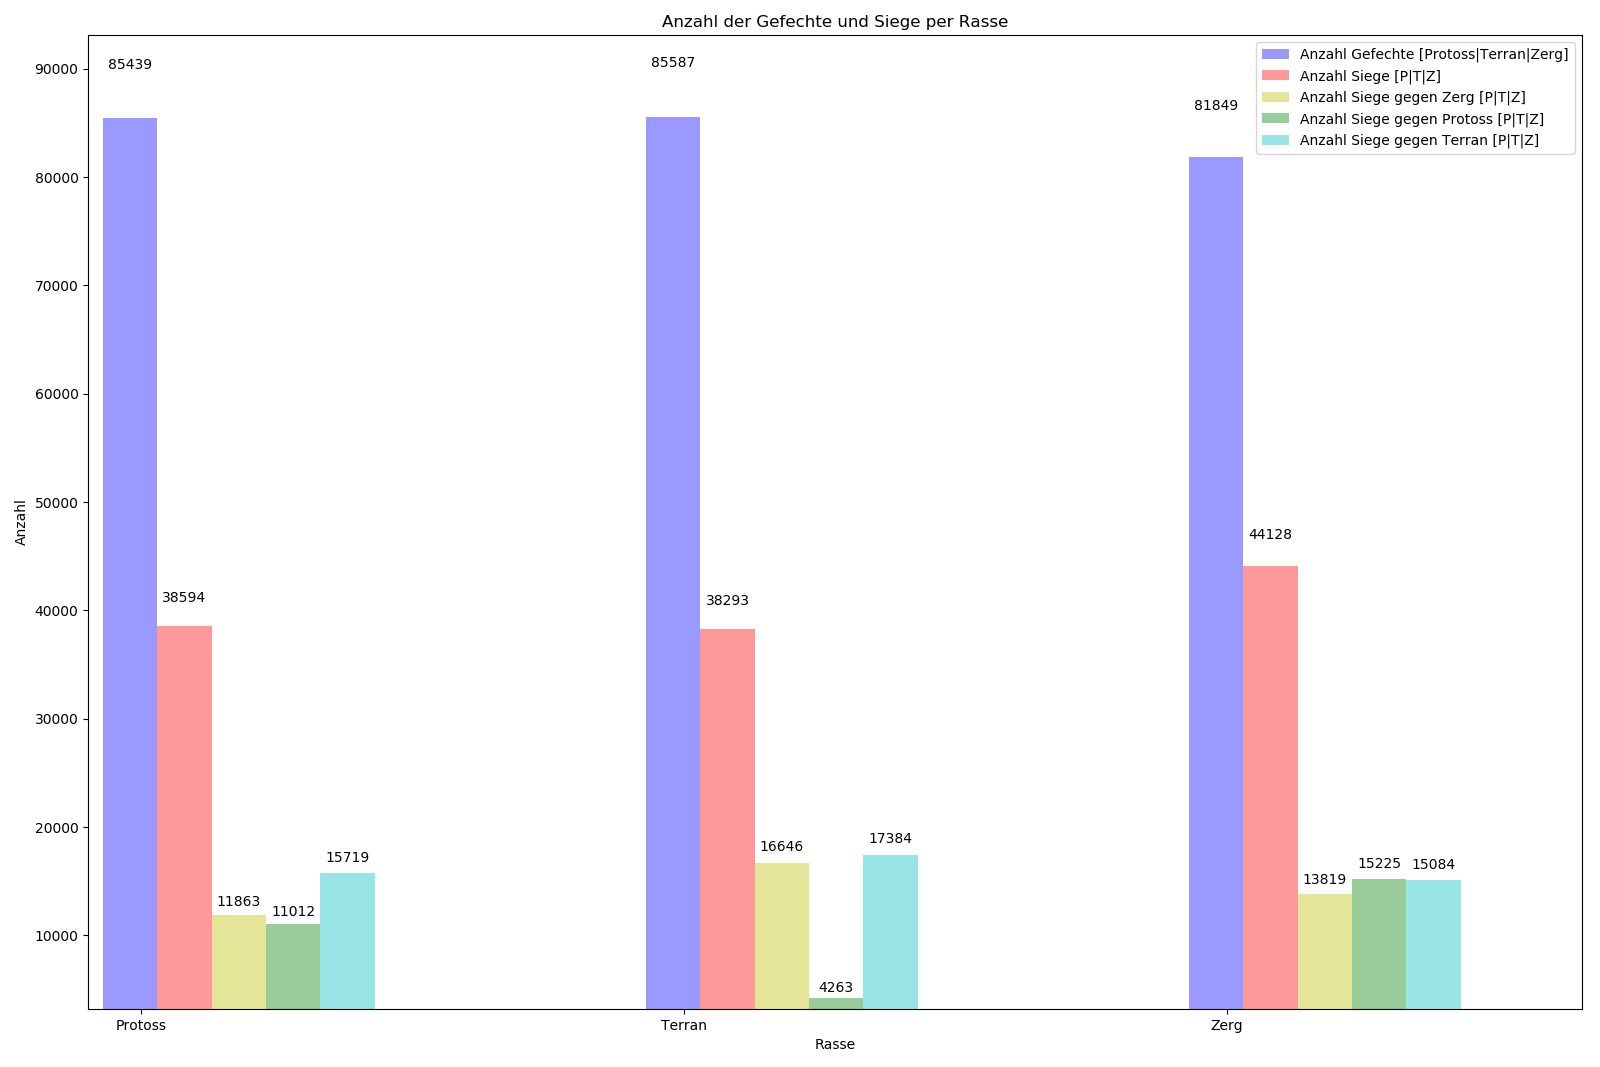
\includegraphics[scale=0.4]{pictures/Graph_Matches_2}
\caption{Verteilung der Siege nach Rasse und Gegnerrasse.}
\label{fig:siegvert}
\end{figure}

In Abbildung \ref{fig:siegsupp} werden die Siege nach Supply-Differenz und Rasse grob unterteilt analysiert. Die Balkengruppen auf der X-Achse bilden die unterschiedlichen Supply-Differenzen ab. Auf der Y-Achse sind die Siege in absoluten  Zahlen aufgetragen. \textit{Sieg bei kleiner Differenz} umfasst alle Siege, bei denen der Sieger einen Supply-Vorteil $sv$ von $ 0 < sv \leq 5$ hatte. \textit{Sieg trotz Nachteil} beinhaltet alle Siege, bei denen der Sieger weniger Supply genutzt hat als der Verlierer. \textit{Siege mit hoher Differenz} zählt alle Siege mit einer Differenz größer 5 auf, bei denen der Sieger im Vorteil war und \textit{Siege bei gleichem Supply} umfasst alle Siege bei denen der Supply exakt gleich war. Anhand der Verteilung der Siege lässt sich ablesen, dass Zerg bei einem Supply-Vorteil zum Sieg tendieren, während Protoss die Besten darin sind, aus einem Nachteil einen Sieg zu machen. Bei gleichem Supply sind die Zerg am schwächsten und Protoss am erfolgreichsten. 


\begin{figure}[H]
\centering
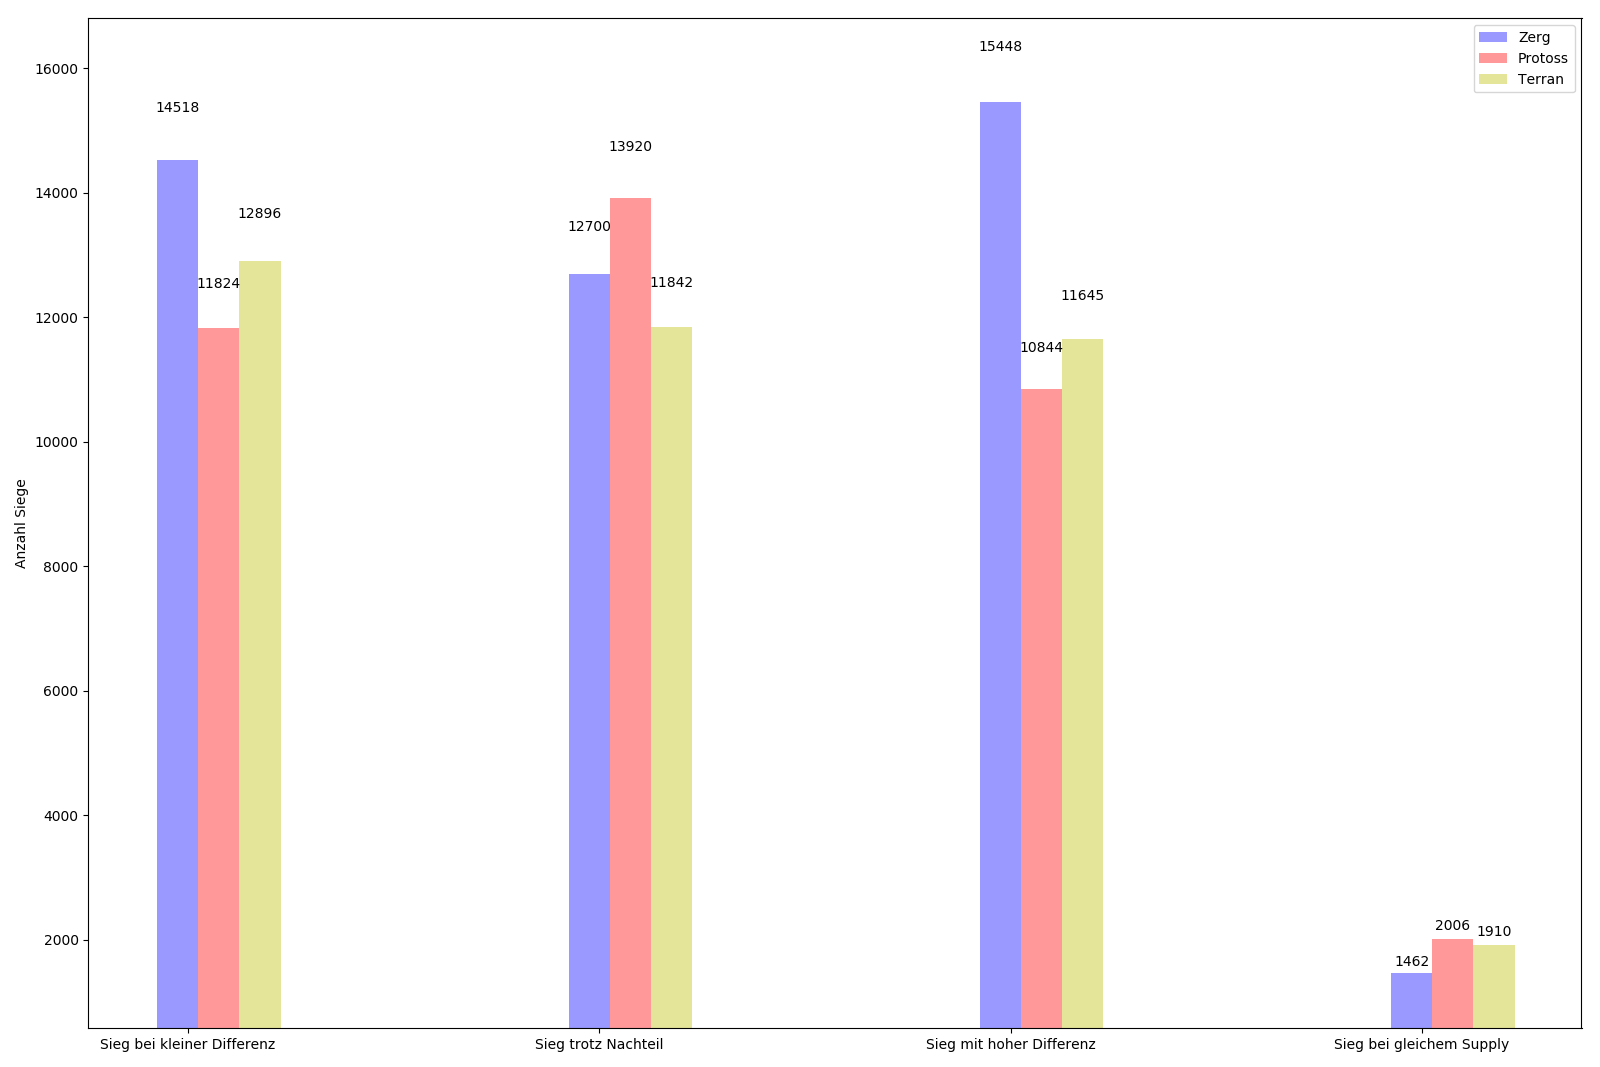
\includegraphics[scale=0.4]{pictures/Graph_Supp_Wins}
\caption{Verteilung der Siege nach Supply-Differenz und Rasse.}
\label{fig:siegsupp}
\end{figure}

\subsection{Evaluationsmetriken}
\label{Metriken}
Die Leistungsfähigkeit der einzelnen Architekturen wird Anhand verschiedener Metriken bestimmt. Die TOP-1 error rate (zu Deutsch: Top-1 Fehlerrate) wird in der aktuellen Forschung häufig zum Vergleich unterschiedlicher Machine Learning Methoden  verwendet. Bei der Klassifizierung von Datensätzen mit einer Vielzahl an Klassen wird im Regelfall die TOP-5 zusätzlich verwendet. Da sich das Klassifizierungsproblem in dieser Arbeit auf drei Klassen beschränkt, entfällt diese Möglichkeit. Die TOP-1 error rate beschreibt bei wie vielen Klassifizierungen das Neural Network die falsche Klasse vorhergesagt hat und steht im direkten Verhältnis zur Accuracy, welche beschreibt wie viele Klassen korrekt vorhergesagt wurden. Es gilt also:
\begin{equation}
TOP\text{-}1 = Vorhersagen_{Falsch} \div Vorhersagen_{Gesamt}
\end{equation}
\begin{equation}
Accuracy = Vorhersagen_{Wahr} \div Vorhersagen_{Gesamt}
\end{equation}
\begin{equation}
Accuracy = 1 \; - \; TOP\text{-}1
\end{equation}

Neben der TOP-1 error rate wird die Leistung der Architekturen auch mit den Metriken Precision (zu Deutsch: Präzision), Recall (zu Deutsch etwa: Widerruf) und F1-Score bemessen. Die für diese Metriken relevanten Teile der Klassifizierung sind in den Abbildungen \ref{fig:prerec} und \ref{fig:prerecacc} dargestellt. Abbildung \ref{fig:prerec} zeigt die Verteilung der Daten nach der Vorhersage durch den Klassifizierungsalgorithmus. Im Kreis berfinden sich alle Datenpunkte, welche der Algorithmus als \textit{Wahr} vorhergesagt hat. Außerhalb finden sich alle Punkte wieder, die als \textit{Falsch} klassifiziert wurden. Alle Punkte auf der linken Hälfte des Bildes sind eigentlich \textit{Wahr} und somit relevant für die Klassifizierung, während sich auf der rechten Seite ausschließlich falsche und somit irrelevante Datenpunkte befinden. Daher gelten alle Punkte auf der linken Seite  außerhalb des Kreises als (\textit{False negative}) und alle Punkte innerhalb des Kreises als (\textit{True positive}). Auf der rechten Seite gilt dementsprechend, dass die Daten im Kreis (\textit{False positive}) und die Punkte außerhalb  (\textit{True negative}) sind. Abbildung \ref{fig:prerecacc} zeigt nun die daraus resultierende Berechnung der unterschiedlichen Metriken. Precision errechnet sich aus dem Verhältnis der \textit{True positive} Daten zu der Gesamtheit der positiven Daten $True\,positive + False\,positive$. Die Metrik spiegelt daher wieder sicher ein Algorithmus darin ist Daten richtig zu evaluieren. Die Metrik vernachlässigt jedoch wie hoch der Anteil der positiven Daten ist, der gefunden wird. Beispielsweise könnte ein Algorithmus eine Klasse lediglich ein Mal als richtig bewerten. Liegt er damit richtig so wäre der Precision-Wert 1, da ein \textit{True positive} zusammen mit keinem \textit{False positive} $1 \div (1+0) = 1$ ergibt. Daher wird als zweite Metrik der Recall herangezogen. Dieser errechnet sich aus dem Verhältnis der Anzahl an \textit{True postive} Datenpunkten zu der Anzahl der relevanten Daten $True\,positive + False\,negative$ und veranschaulicht somit wie gut der Algorithmus die richtigen Klassen wiedererkennt. Der Abbildung der Accuracy dient zur Veranschaulichung der Unterschiede der drei Metriken, da in jedem Fall unterschiedliche Datenmengen herangezogen werden. Der F1-Score dient der Zusammenfassung beider Metriken (Precision und Recall), indem er das gewichtete harmonische Mittel abbildet. Der F1-Score errechnet sich wie in Gleichung \ref{eq:f1} beschrieben für $\alpha = 1$ (Gleichung \ref{eq:f1b}). 

\begin{equation}
F_\alpha = (1 + \alpha^2) \cdot (Precision \cdot Recall) \div (\alpha^2 \cdot Precision + Recall) 
\label{eq:f1} 
\end{equation}
\begin{equation}
F_1 = 2 \cdot (Precision \cdot Recall) \div (Precision + Recall) 
\label{eq:f1b} 
\end{equation}
\begin{figure}[H]
\centering
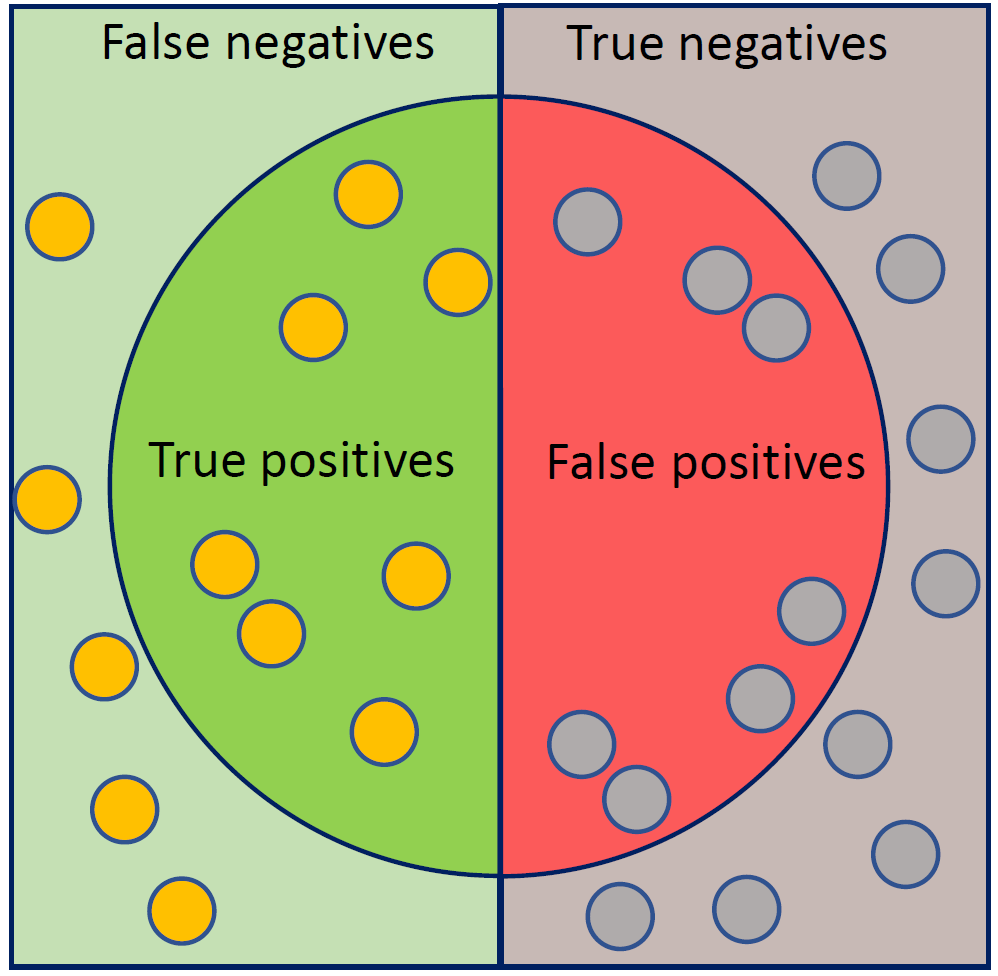
\includegraphics[scale=0.4]{pictures/grafiken/PrecisionRecall}
\caption{Verteilung der relevanten Elemente als Grundlage für Precision und Recall.}
\label{fig:prerec}
\end{figure}
\begin{figure}[H]
\centering
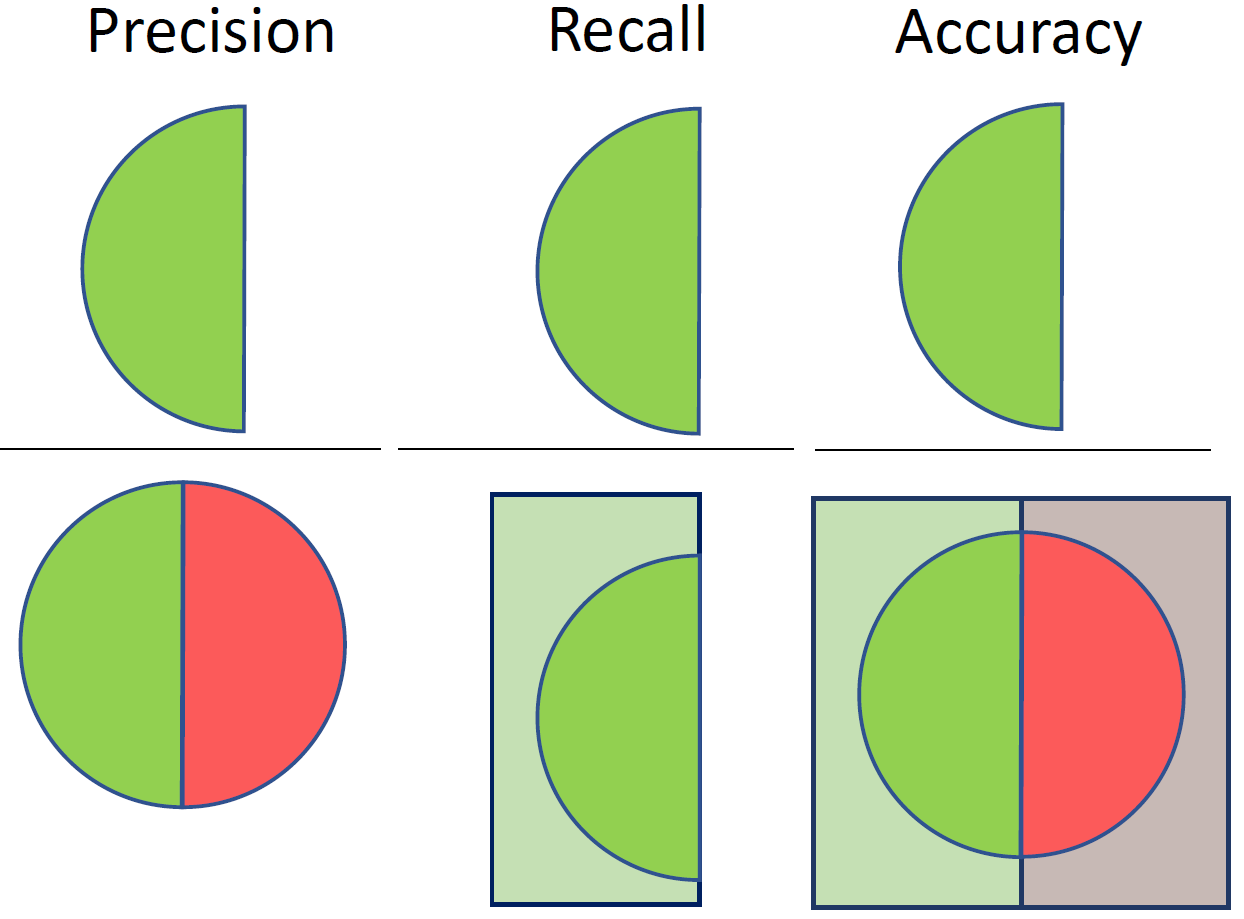
\includegraphics[scale=0.4]{pictures/grafiken/prerecacc}
\caption{Schematische Darstellung der Errechnung von Precision, Recall und Accuracy.}
\label{fig:prerecacc}
\end{figure}

\subsection{Trainingsmethodik}

CNNs können sich diverse Hyperparameter zu nutze machen um den Trainingserfolg zu erhöhen. Außerdem kann mit der Auswahl des Optimierungsalgorithmus (folgend Optimizer) auch Einfluss auf das Lernverhalten der Neural Networks genommen werden. Alle Architekturen verwenden den Adam-Optimizer, welcher in der gängigen Literatur immer wieder Anwendung findet. Der Adam-Optimizer ist ein Algorithmus der die Vorteile von AdaGrad und RMSProp kombiniert \parencite{DBLP:journals/corr/KingmaB14}, indem er jedem Parameter eine Learning Rate (zu Deutsch: Lernrate) zuweist und diese im Verlauf des Trainings anpasst. Der wichtigste Hyperparameter in dieser Arbeit ist die Learning Rate. Sie bestimmt den Faktor, der bei der Errechnung der Gewichtsanpassungen durch Backpropagation genutzt wird und somit wie stark der Optimizer die Gewichte verändern kann. Die Learning Rate wurde je nach Modell und Aufbau etwas variiert und liegt aber stets zwischen 0,01 und 0,001. Im Laufe des Trainings werden alle Layer mittels der sogenannten \textit{Kernel Regularization} (zu Deutsch etwa: Kern-Normalisierung) normalisiert. Kernel Regularization entspricht einem Hyperparameter, der für jeden Layer eines Neural Networks definiert wird. Dieser Hyperparameter ist ein festgelegter Wert auf die Loss Function addiert wird und die damit die Anpassung der Gewichte beeinflusst. Er soll unter anderem Overfitting verhindern. Für alle Netze wird in jedem Layer die Regularizierung mittels L2 regularization mit dem Wert  $1\times e^{-4}$. Für alle K Die Inception-SE-Architektur fordert zudem mit der Reduction Ratio (Reduktionsverhältnis) einen weiteren Hyperparameter. Dieser steuert den Zuwachs an Parametern durch die Fully-Connected Layer im Squeeze-and-Excitation Block der Architektur und sein Wert liegt in dieser bei 4. Das bedeutet, dass in dem ersten Fully-Connected Layer die Anzahl der Channel durch 4 geteilt wird um die Dimensionen der Ausgabe zu reduzieren und somit die Anzahl der benötigten Parameter zu verkleinern. 

In dem Trainingsvorgang wird Data Augmentation (zu Deutsch: Datenvermehrung) verwendet. Dieser Vorgang verfolgt zwei Ziele. Zum einen soll die Anzahl der verfügbaren Daten erhöht werden, zum anderen sollen die Architekturen die Stärke der Armeen unabhängig von ihrer Lage auf dem Schlachtfeld evaluieren können. Beides wird angegangen indem alle Eingabematrizen in vier Versionen jeweils 90 Grad rotiert in den Datensatz eingespeist werden (folgend: Rotated-Variante). So muss die Architektur das Gefecht in vier Richtungen analysieren und ist gezwungen den Werten der Armeen eine höhere Aufmerksamkeit zu schenken. Als zweite Augmentierungsmethode wurden die Matrizen nur einmal dupliziert und um 180 Grad rotiert (folgend: Mirrored-Variante). Zusätzlich wurden die Label getauscht. Neben der Datenvermehrung, soll so überprüft werden, ob sich die Architekturen bei der Vorhersage der Gewinnerseite anders verhalten, oder ob ähnliche Ergebnisse zu erwarten sind.


Im Zuge der Evaluierung aller Architekturen wurde jede Architektur mit beiden Augmentierungsvarianten und einer Version ohne Augmentierung (folgend: NoAug-Variante) analysiert. 

Die vorgestellte ResNet-Architektur wurde mit jeweils 90.000 Datensätzen für die Rotated-Variante und 30.000 Datensätzen für die Mirrored-Variante und die NoAug-Variante trainiert. Die NoAug-Variante wurde mit einer Learning Rate von 0,001 trainiert, die Rotated-Variante mit 0,01 und die Mirrored-Variante mit 0,005. Abbildung \ref{fig:resnet_loss} zeigt den Verlauf der Verlustfunktion während des Trainings für alle drei Varianten. Sowohl bei der Rotated- als auch bei der Mirrored-Variante findet man einen plötzlichen Anstieg der Verlustwerte im Verlauf des Trainings. Dieser Ausschlag geht damit einher, dass das Netz ab einem bestimmten Zeitpunkt alle Daten zur selben Klasse evaluiert. Da die Mirrored-Variante vor dem Ausschlag die höchste Accuracy aufweist, wird das Modell aus Epoche 17 zur weiteren Auswertung genutzt.

\begin{figure}[H]
\centering
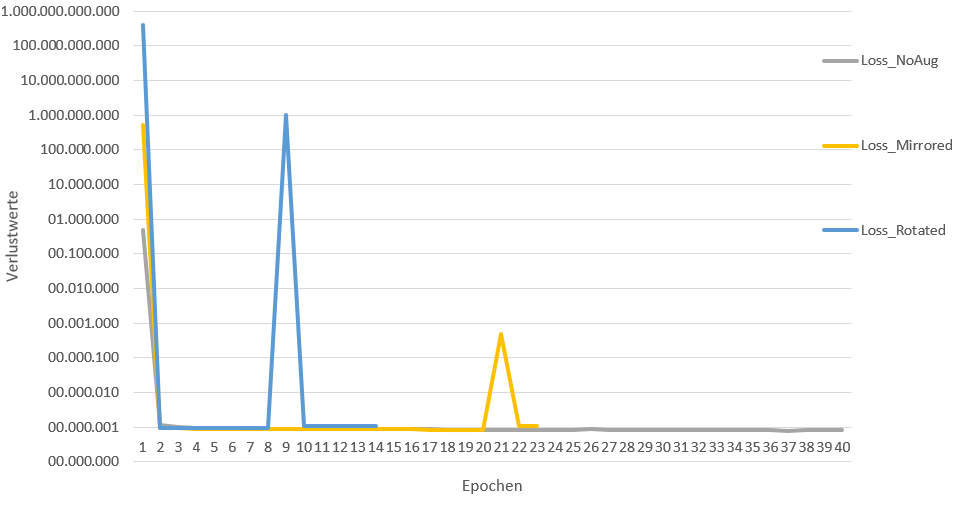
\includegraphics[scale=0.5]{pictures/Auswertung/resnet_loss}

\caption{Verlustwerte der drei ResNet-Varianten.}
\label{fig:resnet_loss}
\end{figure}

Das All-Convolutional Net wurde in allen Varianten mit einer Learning Rate von 0,005 trainiert. Die Rotated-Variante und die Mirrored-Variante wurden mit 90.000 Datensätzen trainiert, die NoAug-Variante wurde aus Zeitgründen mit 30.000 Datensätzen. In Abbildung \ref{fig:loss_allconv} werden die Verlustwerte aller Versionen dargestellt. Es zeigt sich ein fortlaufender Abstieg der Verlustwerte, was andeutet das, alle Varianten auf den Trainingsdaten gute Ergebnisse erzielen. Zieht man mit Abbildung \ref{fig:acc_allconv} allerdings die Accuracy der Testdaten mit in Betracht, so zeigt sich dass alle Varianten nach der 10 Epoche zum Overfitten neigen. Es wird die Mirrored-Variante, zur weiteren Evaluierung herangezogen, da sie auf den Testdaten die beste Accuracy aufwies. 

\begin{figure}[H]
\centering
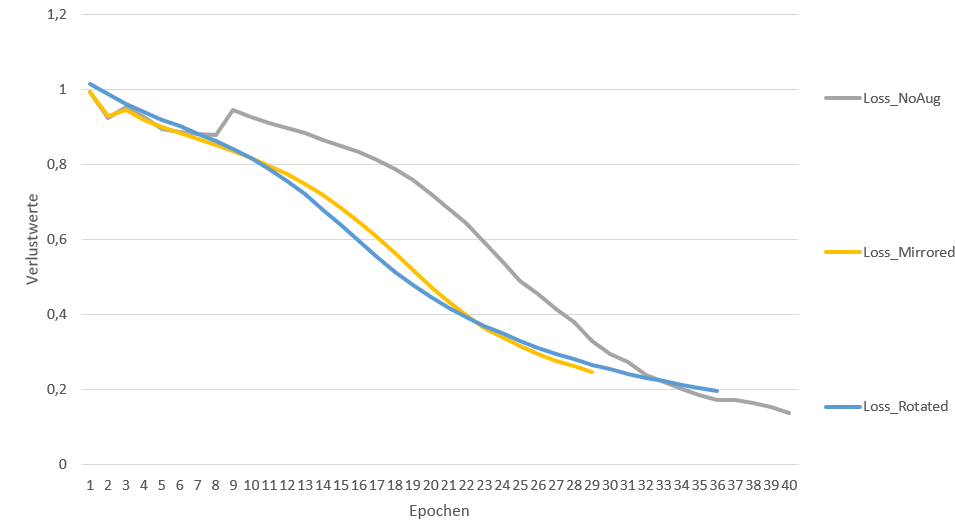
\includegraphics[scale=0.5]{pictures/Auswertung/all_conv_loss}
\caption{Entwicklung der Verlustwerte der All-Convolutional Net-Varianten während des Trainings.}
\label{fig:loss_allconv}
\end{figure}
\begin{figure}[H]
\centering
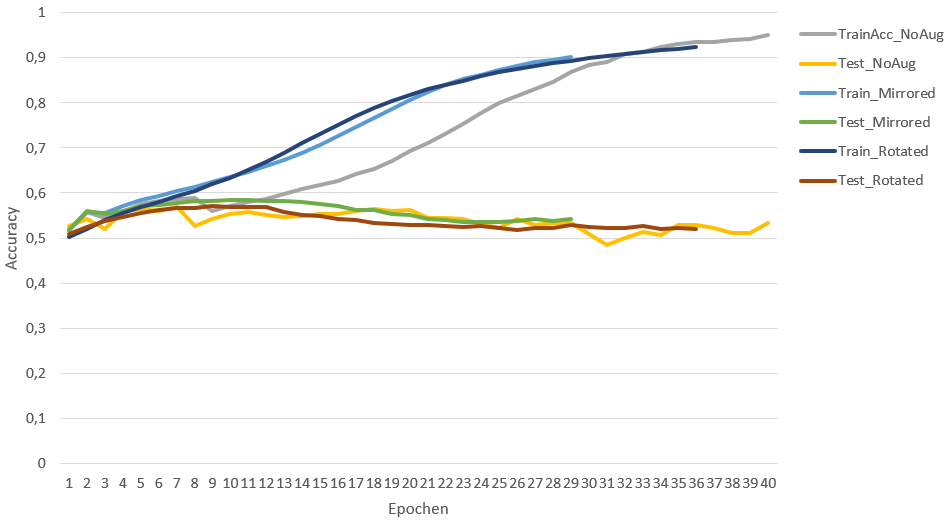
\includegraphics[scale=0.5]{pictures/Auswertung/all_conv_acc_}
\caption{Entwicklung der Accuracy aller All-Convolutional Net-Varianten für Test- und Trainingsdaten.}
\label{fig:acc_allconv}
\end{figure}

\paragraph{Inception V4}

Inception V4 wurde mit der Learning Rate 0,001 trainiert. Auf der Abbildung \ref{}**TBD** sind die Werte der Accuracy aller Versionen eingetragen. Die X-Achse zeigt die Epochen und die Y-Achse stellt die Accuracy-Werte dar. In der Abbildung sind zwei Durchläufe ohne Augmentierung in blau (a) und orange (b) enthalten, sowie ein Durchgang mit 90 Grad Rotation in **TBD** (c) und ein Durchgang mit 180 Grad Rotation in **TBD** (d). Version (a) wurde mit 90.000 Datensätzen trainiert, während (b) lediglich mit 60.000 Datensätzen trainiert wurde. 
Die Versionen (a) und (b) zeigen einen ähnlichen Verlauf und tendieren zum Overfitten. (a) hat im Testdatensatz sein Maximum in Epoche 10 bei 0,5739. (b) findet sein Maximum eine Epoche später in Epoche 11 mit einem Wert von 0,5690. Beide Durchgänge folgen dem bei All-Convolutional Nets beschriebenen Muster des Overfittens, indem bei beiden Netzen nach erreichen der Maxima Test- und Trainings-Accuracy auseinandergehen. Während sich die Trainings-Accuracy erneut dem Wert 1 annähert schwankt die Test-Accuracy in beiden Fällen zwischen 0,50 und 0,53.

**TBD**
Bild mit den Accuracies von Inception V4
**TBD**
 
\paragraph{Inception mit Squeeze-and-Excitation-Layer}

\subsection{Resultate}
\label{Resultate}

\begin{table}
\centering
\caption{Auflistung der Accuracy und des F1-Score auf den Testdaten für alle Architekturen.}
\begin{tabular}{@{}lrr@{}}
\hline
Architektur & Accuracy & F1-Score\\
\hline
All-Convolutional Net & 0,585 & 0,567\\
ResNet & 0,611 & 0,601\\
Inception V4 & & \\
Inception V4 SE & & \\
\hline
\end{tabular}
\label{tb:resnet}
\end{table}